\section{Electric Fields}



\subsection{electric forces \& fields}

\subsubsection{electrostatic forces}

any charged object can interact with any other charged object

this force is known as the \emph{electrostatic force}, or in short, the electric force

\cmt electric force can be \emph{repulsive} or \emph{attractive}, depending on nature of charge

like charges would repel, opposite charges would attract



\subsubsection{electric fields}

charged objects can interact without physically touching each other 

to explain this \emph{action at a distance}, we introduce the concept of \emph{force fields}

a force field is basically a region of space where a body experiences a force
\footnote{Apart from electric fields (act on bodies carrying electric charges), other examples of force fields in physics are gravitational fields (act on objects with mass) and magnetic fields (act on magnets, electric currents or moving charges). You will be studying these subjects at A-Levels.}

\begin{ilight}
	\centering \keypoint{electric field} is a region of space in which a charged object is acted by an electric force\index{electric field!electric field}
\end{ilight}

to elaborate, any charged body can create an electric field around it

property of space is altered, so another charged body in the field experiences a force

from this point of view, when charged bodies interact, they do not directly exert forces upon each other, but they interact through electric fields







\newpage

\subsubsection{electric field strength}

to describe how strong an electric field is at a point, we define the \emph{electric field strength}\index{electric field!electric field strength}

\begin{ilight}
	\centering \keypoint{electric field strength} is the electric force acting per unit positive charge: $\boxed{E = \frac{F}{q}}$
\end{ilight}

\cmt SI unit of electric field strength: $[E] = \text{N C}^{-1} = \text{V m}^{-1}$

\cmt electric field strength is a vector quantity

direction of field strength is defined as the force experienced by a \emph{positive} test charge


\cmt given the field strength $E$, electric force on a test charge $q$ can be determined

\begin{wrapfigure}{r}{0.4\textwidth}
	\vspace*{-5pt}
	\centering
	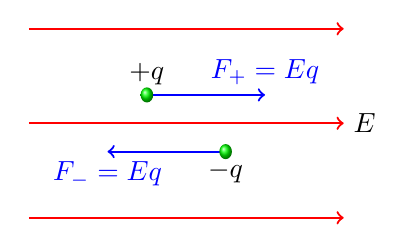
\begin{tikzpicture}[yscale=1.2]
	\foreach \x in {1,2,3} \draw[red,thick,->] (0,\x) -- (4,\x);
	\node[right] at (4,2) {$E$};
	\draw[blue,thick,->] (1.5,2.3) -- ++ (1.5,0) node[above]{$F_+=Eq$};
	\shade [ball color = green] (1.5,2.3) circle (0.08) node[above]{$+q$};
	\draw[blue,thick,->] (2.5,1.7) -- ++ (-1.5,0) node[below]{$F_-=Eq$};
	\shade [ball color = green] (2.5,1.7) circle (0.08) node[below]{$-q$};
	\end{tikzpicture}
	\vspace*{-16pt}
\end{wrapfigure}

magnitude of electric force is given by $F=Eq$

direction of electric force depends on both direction of $E$ and polarity of $q$

\begin{compactitem}
	\item[--] for positive charge, $F$ is in same direction as $E$
	
	\item[--] for negative charge, $F$ is in opposite direction as $E$
\end{compactitem}


\cmt  electric fields due to two (or more) different sources can overlap

the combined field strength is \emph{vector sum} of the individual fields

%\example{An electron is at a point where the electric field strength is 1500 N C$^{-1}$, what is the electric force acting on the electron?}
%
%\solc\begin{equation*}
%	F = Eq = 1500 \times 1.60 \times 10^{-19} \RA F = 2.4 \times 10^{-16} \text{ N} \teoe
%\end{equation*}





\subsubsection{electric field lines}

pattern of an electric field can be graphically represented by \keypoint{electric field lines}\index{electric field!field lines}

\cmt field lines can give information about electric field strength

\begin{compactitem}
	\item[--] tangents of the field lines point in same direction as field strength
	
	\item[--] density of the lines gives information about magnitude of field strength
\end{compactitem}

\cmt some rules for drawing electric field lines are given below

\begin{compactitem}
	\item[--] field line starts radially outwards from a positive charge (or from infinity)
	
	\item[--] field line ends up radially inwards on a negative charge (or to infinity)
	
	\item[--] field lines can never intersect each other\footnote{This is because $E$ at a given position must point in a definite direction unless it is zero.}
	
	\item[--] filed lines are always perpendicular to the surface of a conductor\footnote{This is because $E=0$ everywhere inside a conductor, so field strength cannot have components that are tangent to a conducting surface.}
\end{compactitem}




\example{The diagrams below show the pattern of various electric fields.}

\begin{figure}[htp]
	\centering
	\begin{minipage}{0.45\linewidth}
		\centering
		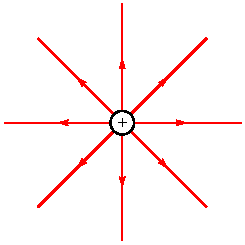
\includegraphics[height=96pt]{pos-charge}
	\end{minipage}
	\begin{minipage}{0.45\linewidth}
		\centering
		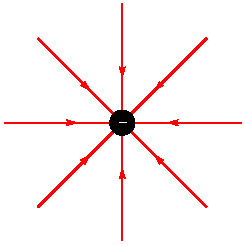
\includegraphics[height=96pt]{neg-charge}
	\end{minipage}
	
	\begin{center}
		radial fields around (a) an isolated positive charge, (b) an isolated negative charge
	\end{center}
\end{figure}

\begin{figure}[htp]
	\vspace*{-18pt}
	\begin{minipage}{0.3\linewidth}
		\centering
		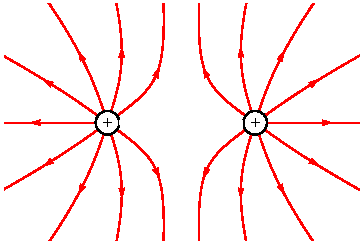
\includegraphics[height=96pt]{like-charges}
	\end{minipage}\hfill
	\begin{minipage}{0.3\linewidth}
		\centering
		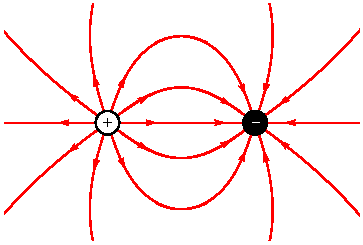
\includegraphics[height=96pt]{opposite-charges}
	\end{minipage}\hfill
	\begin{minipage}{0.3\linewidth}
		\centering
		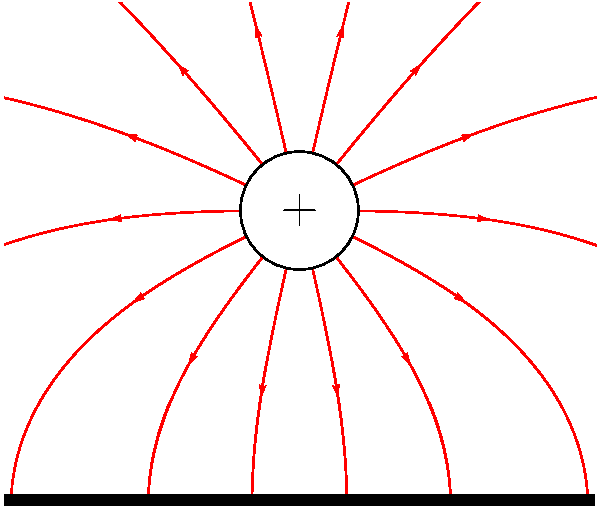
\includegraphics[height=96pt]{sheet-charge}
	\end{minipage}
	
	\begin{center}
		field between (c) two equal and like charges, (d) two equal but opposite charges,
		
		(e) a positive charge and a large conducting sheet that is earthed
	\end{center}
	
	
\end{figure}


\subsection{uniform electric fields}

\begin{wrapfigure}{R}{0.4\textwidth}
	\vspace{-12pt}
	\begin{center}
		\begin{circuitikz}[european resistors,xscale=0.95]
		\draw[thick] (-1.8,-1) -- (1.8,-1) (-1.8,1) -- (1.8,1);
		\draw[thick] (0,-1) -- (0,-2) node[midway,left]{\Large$-$} -- (3.2,-2)  (3.2,2) -- (0,2) -- (0,1)  node[midway,left]{\Large$+$};
		\draw[thick] (3.2,2) to[battery,l^=$V$] (3.2,-2);
		\foreach \x in {-1.5,-0.5,0.5,1.5} \draw[red,->] (\x,1) -- (\x,-1);
		\draw[<->] (2,-1) -- (2,1) node[midway,right]{$d$};
		\node[purple] at (0,0) {$E$};
		\end{circuitikz}
	\end{center}
	\vspace{-20pt}
\end{wrapfigure}

let's take two parallel metal plates and connect them to a high-voltage supply as shown

a charge in the region between the plates experiences a constant force regardless of its location in the field

field strength is constant throughout the region

this field is said to be a \keypoint{uniform electric field}\index{electric field!uniform electric field}

field lines of a uniform field are a set of parallel lines of equal spacing as shown on the right



\cmt if the two plates are separated by a distance of $d$, and a p.d. of $V$ is applied across them

then magnitude of field strength of the uniform field is given by: $\boxed{ E = \frac{V}{d}}$

\noindent\textbf{proof:} work done to bring a test charge $q$ from positive plate to negative plate: $ W=Fd=Eqd $

the change in electric potential energy is: $ \Delta E_p = q V$ (check \S\ref{ch:potential-difference} for meaning of p.d.)

work-energy theorem tells us these two must be equal: $ Eqd = qV$, so we find: $ {E=\frac{V}{d}} $


\cmt electric field between metal plates points from high potential towards low potential

\example{The following examples show the set-up of two uniform electric fields.}

\begin{figure}[ht]
	\centering
	\begin{minipage}{0.45\textwidth}
		\centering
		\begin{tikzpicture}
		\draw[thick] (-1.8,-1) -- (1.8,-1) (-1.8,1) -- (1.8,1);
		\draw[thick,white] (0,-1) -- (0,-1.1) node[ground]{};
		\draw[thick] (0,-1) -- (0,-1.5) node[below]{$-50$ V} (0,1.5) node[above]{$+30$ V} -- (0,1)  ;
		\foreach \x in {-1.5,-0.5,0.5,1.5} \draw[red,->] (\x,1) -- (\x,-1);
		\draw[<->] (2.25,-1) -- (2.25,1) node[midway,right]{10 cm};
		\node[purple] at (0,0) {$E$};
		\end{tikzpicture}
		\begin{equation*}
			E = \frac{V}{d} = \frac{(+30)-(-50)}{0.10} = 800\NpC
		\end{equation*}
	\end{minipage}\hfil
	\begin{minipage}{0.45\textwidth}
		\centering
		\begin{tikzpicture}
		\draw[thick] (-1.8,-1) -- (1.8,-1) (-1.8,1) -- (1.8,1);
		\draw[thick,white] (0,-1) -- (0,-1.5) node[below]{$-50$ V} (0,1.5) node[above]{$+30$ V} -- (0,1)  ;
		\draw[thick] (0,-1) -- (0,-1.1) node[ground]{} (0,1.5) node[above]{$-60$ V} -- (0,1) ;
		\node[right] at (0.3,-1.55) {earthed ($V_0=0$)};
		\foreach \x in {-1.5,-0.5,0.5,1.5} \draw[red,<-] (\x,1) -- (\x,-1);
		\draw[<->] (2.25,-1) -- (2.25,1) node[midway,right]{12 cm};
		\node[purple] at (0,0) {$E$};
		\end{tikzpicture}
		\begin{equation*}
		E = \frac{V}{d} = \frac{0-(-60)}{0.12} = 500\NpC
		\end{equation*}
	\end{minipage}
\end{figure}


\example{Two horizontal parallel plate conductors are separated by 1.5 cm in air. A potential difference of 36 V is applied across the plates. Compare the electric force and gravitational force acting on a proton between the plates.}

\sol electric field strength: $E = \frac{V}{d} = \frac{36}{1.5\times10^{-2}} = 2400 \NpC$

electric force: $F_E = Eq = 2400 \times 1.60\times10^{-19} \approx 3.84\times10^{-16} \text{ N}$

weight of the proton: $W = mg = 1.67\times10^{-27} \times 9.81 \approx 1.64\times10^{-26} \text{ N}$

this shows electric force on proton are much stronger than gravitational forces

when dealing with motion of sub-atomic particles (e.g., protons, electrons, etc.) in an electric field, effects of gravity can therefore be ignored \eoe



\subsubsection{equilibrium between electric force and weight}


\begin{wrapfigure}{R}{0.36\textwidth}
	\vspace{-16pt}
	\begin{center}
		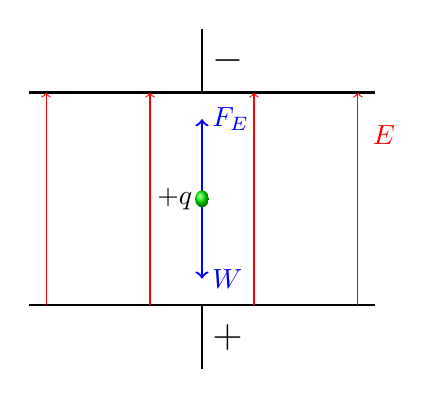
\begin{tikzpicture}[xscale=1.1,yscale=1.35]
		\draw[thick] (-2,-1) -- (2,-1) (-2,1) -- (2,1);
		\draw[thick] (0,-1.6) -- (0,-1) node[midway,right]{\Large$+$} (0,1) -- (0,1.6) node[midway,right]{\Large$-$};
		\foreach \x in {-1.8,-0.6,0.6,1.8} \draw[red,->] (\x,-1) -- (\x,1);
		\draw[blue,thick,->] (0,0) -- (0,-0.75) node[right]{$W$};
		\draw[blue,thick,->] (0,0) -- (0,0.75) node[right]{$F_E$};
		\shade [ball color = green] (0,0) circle (0.08) node[left]{$+q$};
		\node[red] at (2.1,0.6) {$E$};
		\end{tikzpicture}
	\end{center}
	\vspace{-20pt}
\end{wrapfigure}

a charged particle (e.g., a dust particle or an oil droplet) can be held stationary in a uniform electric field

electric force is in equilibrium with weight of particle

{
	\centering
	
	$ F_E = W \RA Eq = mg $
	
}

\noindent where field strength $E$ is given by: $E = \frac{V}{d}$

note that equilibrium is possible only if $F_E$ acts in opposite direction to $W$, so direction of the applied field depends on polarity of the charged particle



\newpage


\example{A uniform electric field is set up between the two parallel oppositely-charged metal plates separated by 8.0 cm. An oil droplet of mass 0.040 g and charge $-20$ nC is placed in the field. The droplet stays at rest. (a) Find the strength and the direction of the electric field. (b) What is the voltage required to produce this field? (c) If the separation between the plates is reduced, what would happen to the oil droplet?}

\sol (a) equilibrium so electric force equals weight: $F_E = mg = 0.050 \times 10^{-3} \times 9.81 \approx 3.92 \times 10^{-4} \text{ N}$

\hspace*{1.2em} field strength: $E = \frac{F_E}{q} = \frac{ 3.92 \times 10^{-4} }{ 20 \times 10^{-9}} \approx 1.96 \times 10^{4} \NpC$

\hspace*{1.2em} $F_E$ must act upwards for equilibrium, but droplet is negatively-charged

\hspace*{1.2em} so electric field acts in the downward direction

(b) voltage between the plates: $V = E d = 1.96 \times 10^{4} \times 8.0 \times 10^{-2} \approx 1.57 \times 10^3 \text{ V}$

(c) smaller separation means greater field strength, so greater electric force

\hspace*{1.2em} $F_E > mg$ so resultant force acts upwards, droplet will accelerate upwards \eoe



\subsubsection{deflection of charged particle in uniform fields}

\begin{wrapfigure}{R}{0.4\textwidth}
	\vspace{-21pt}
	\begin{center}
		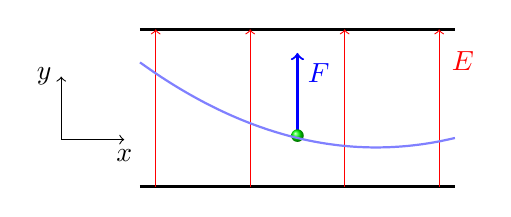
\begin{tikzpicture}[scale=1]
		\draw[very thick] (-2,-1) -- (2,-1) (-2,1) -- (2,1);
		\foreach \x in {-1.8,-0.6,0.6,1.8} \draw[red,->] (\x,-1) -- (\x,1);
		\draw[thick,blue,->] (0,-0.35) -- (0,0.7) node[below right]{$F$};
		\shade [ball color = green,dashed] (0,-0.35) circle (0.08);
		\draw [thick,blue!50,domain=-2:2,samples=20,smooth,variable=\x] plot (\x,{0.12*(\x-1)*(\x-1)-0.5});
		\node[red] at (2.1,0.6) {$E$};
		\draw[<->] (-3,0.4) node[left]{$y$} -- (-3,-0.4) -- (-2.2,-0.4) node[below]{$x$};
		\end{tikzpicture}
	\end{center}
	\vspace{-15pt}
\end{wrapfigure}

charged particle travelling in a uniform electric field would in general undergo a \emph{projectile-like} motion

we set up the coordinates such that electric field is along the $y$-axis, and $x$-axis is in the normal direction

we denote $x_0$, $y_0$ and $u_x$, $u_y$ as initial displacements and initial velocities at $t=0$

electric force only acts in $y$-direction, no force acts in $x$-direction

\begin{compactenum}
	\item[--] in $x$-direction, particle maintains a constant velocity: $v_x = u_x$, $\,\, x = x_0 + u_x t$
	
	\item[--] in $y$-direction, particle accelerates uniformly: $v_y = u_y + a t$, $\,\, y=y_0 + u_y t + \frac{1}{2}at^2$
	
	where acceleration in $y$-direction is given by $ a=\frac{F}{m} = \frac{Eq}{m} \,\,$ (assuming weight is negligible)
\end{compactenum}

so motion of a charged particle in a uniform electric field is analogous with projectile motion in a uniform gravitational field (see \S\ref{ch:projectile}), i.e., trajectory of charged particle is \emph{parabolic}


\begin{wrapfigure}{R}{0.54\textwidth}
	\vspace{-15pt}
	\begin{center}
		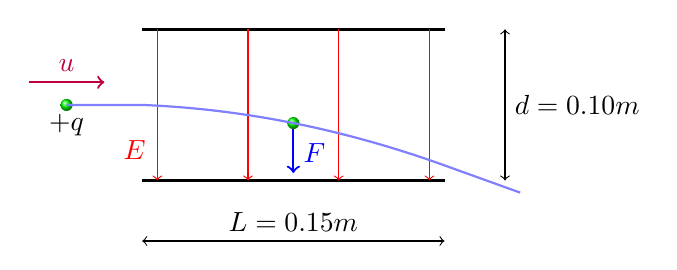
\begin{tikzpicture}[scale=.96]
		\draw[very thick] (-2,-1) -- (2,-1) (-2,1) -- (2,1);
		\draw[<->] (-2,-1.8) -- (2,-1.8) node[midway,above] {$L=0.15 \text{ m}$};
		\draw[<->] (2.8,-1) -- (2.8,1) node[midway,right] {$d=0.10 \text{ m}$};
		\foreach \x in {-1.8,-0.6,0.6,1.8} \draw[red,<-] (\x,-1) -- (\x,1);
		\shade [ball color = green] (-3,0) circle (0.08) node[below]{$+q$};
		\draw[thick,blue,->] (0,-0.24) -- (0,-0.9) node[above right]{$F$};
		\shade [ball color = green,dashed] (0,-0.24) circle (0.08);
		\draw[->,thick,purple] (-3.5,0.3) -- (-2.5,0.3) node[midway,above]{$u$};
		\draw [thick,blue!50,domain=-2:2,samples=20,smooth,variable=\x] plot (\x,{-0.04*(\x+2.5)*(\x+2.5)+0.01}) (-2.0,0) -- (-3,0) (2.0,-0.8) -- ++(1,-0.36);
		\node[red] at (-2.1,-0.6) {$E$};
		\end{tikzpicture}
	\end{center}
	\vspace{-18pt}
\end{wrapfigure}

\example{A proton enters a uniform field of strength $1.0\times10^4\NpC$ at an initial velocity of $5.0\times10^5\mps$. The initial direction of motion is at right angles to the field. The dimensions of the field are shown in the diagram. (a) What is the time taken for the proton to pass through the field? (b) What is the deviation in the direction of the field during this time? (c) If an electron enters the field with the same initial velocity, describe how the deflection of the electron compares with that of the proton.}

\sol constant horizontal velocity, so time taken: $t = \frac{L}{u} = \frac{0.15}{5.0\times10^5} = 3.0\times10^{-7} \text{ s}$

\eqyskip constant acceleration in direction of field: $
a = \frac{F}{m} = \frac{Eq}{m} = \frac{1.0\times10^4\times1.6\times10^{-19}}{1.67\times10^{-27}} \approx 9.58\times10^{11}\mpss $

\eqyskip displacement moved in this direction: $
\Delta y=\frac{1}{2}at^2 = \frac{1}{2} \times 9.58\times10^{11} \times (3.0\times10^{-7})^2 \approx 0.043 \text{ m} $

electron would experience a much greater deflection in the opposite direction

\begin{compactenum}
	\item[--] electron has opposite charge to proton, so deflect in the opposite direction
	
	\item[--] mass of electron is much smaller, so much greater acceleration
	
	time spent in the field is the same, so electron has much greater deflection \eoe
\end{compactenum}




\subsubsection{polar molecules in uniform electric fields}

centre of positive and negative charges for a molecule do not necessarily overlap

this molecule is still electrically neutral, i.e., it has a zero net charge

such a molecule is called a \emph{polar molecule}, and it could be affected by an electric field 


\begin{wrapfigure}{R}{0.375\textwidth}
	\vspace{-24pt}
	\begin{center}
		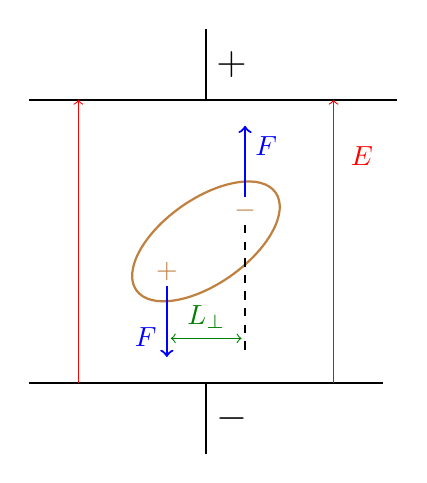
\begin{tikzpicture}[scale=1.8]
		\draw[thick] (-1.25,-1) -- (1.25,-1) (-1.25,1) -- (1.35,1);
		\draw[thick] (0,-1.5) -- (0,-1) node[midway,right]{\Large$-$} (0,1) -- (0,1.5) node[midway,right]{\Large$+$};
		\foreach \x in {-.9,.9} \draw[red,->] (\x,-1) -- (\x,1);
		\node[red] at (1.1,0.6) {$E$};
		\draw[brown,thick,rotate=35] (0,0) ellipse (0.6 and 0.3);
		\node[brown] at (38:0.35) {$-$};
		\node[brown] at (218:0.35) {$+$};
		\draw[thick, blue,->] (38:0.35) ++ (0,0.1) --++ (0,0.5) node[below right]{$F$};
		\draw[thick, blue,->] (218:0.35) ++ (0,-0.1) --++ (0,-0.5) node[above left]{$F$};
		\draw [dashed] (38:0.35) ++ (0,-0.1) --++ (0,-0.9);
		\draw [Green, <->] (38:0.35) ++ (-0.024,-0.9) --++ (-0.5,0) node[midway, above]{$L_\perp$};
		\end{tikzpicture}
	\end{center}
	\vspace{-20pt}
\end{wrapfigure}

the diagram shows a polar molecule in a uniform field

force on centre of positive charge and force on centre of negative charge are labelled as shown

this is a pair of equal but opposite forces

so they give rise to a resultant \emph{torque/moment}

recall \emph{torque of couple} is defined as one force times perpendicular distance between the force pair (see \S\ref{ch:torque-of-couple})

{
	\centering
	
	$\tau = F_E L_\perp \RA \tau Eq L_\perp$
	
}

this torque would cause the polar molecule to \emph{rotate}

